\documentclass[aspectratio=169]{beamer}

% ---------- Pacotes ----------
\usepackage[brazil]{babel}
\usepackage[T1]{fontenc}
\usepackage[utf8]{inputenc}
\usepackage{lmodern}
\usepackage{amsmath, amssymb}
\usepackage{graphicx}
\usepackage{booktabs}

% ---------- Tema ----------
\usetheme{Madrid}
\usecolortheme{default}
\setbeamertemplate{navigation symbols}{}

% ---------- Metadados ----------
\title{Distributed Machine Learning - Server-based e Peer-to-Peer}
\subtitle{Programação Paralela -- BCC447}
\author{Matheus Peixoto Ribeiro Vieira}
\date{\today}

\begin{document}

% =======================
\begin{frame}
  \titlepage
\end{frame}

% =======================
\section{Gradiente e otimização}

\begin{frame}{Gradiente e otimização}
  Considere uma rede (camada linear):
  \[
    Z = WX + b
  \]
  Objetivo: encontrar os melhores parâmetros \(W\) e \(b\) minimizando a função de perda.

  \vspace{0.4em}
  Atualização por descida do gradiente:
  \[
    \theta_{t+1} = \theta_t - \alpha \,\hat{g}_t
  \]
  \begin{itemize}
    \item \(\hat{g}_t\): gradiente estimado (mini-batch)
    \item \(\alpha\): learning rate
  \end{itemize}
\end{frame}

% =======================
\begin{frame}{SGD é ruidoso}
  Cada mini-batch pode induzir um gradiente diferente, levando a direções ligeiramente distintas.

  \vspace{0.6em}
  \begin{center}
    % Ajuste o caminho conforme seu projeto
    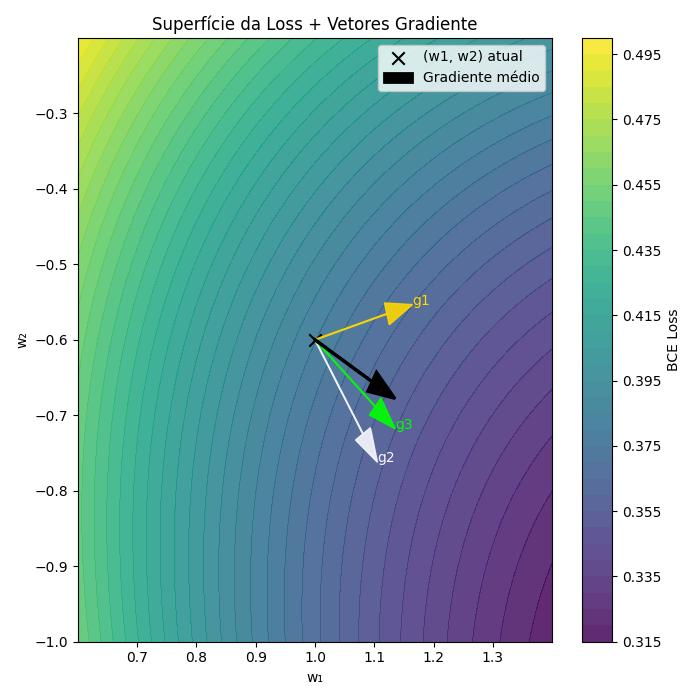
\includegraphics[width=0.50\linewidth]{images/sgd.jpg}
  \end{center}
\end{frame}

% =======================
\section{Acelerando: D-SGD}

\begin{frame}{Acelerando o processo: Distributed SGD (D-SGD)}
  
  \vspace{0.5em}
  \textbf{Fases do D-SGD:}
  \begin{enumerate}
    \item Computação local
    \item Comunicação
    \item Atualização global
  \end{enumerate}

  \vspace{0.6em}
  \begin{center}
    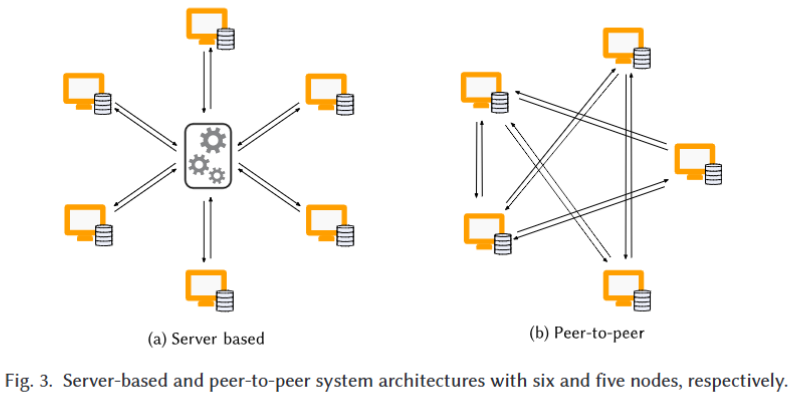
\includegraphics[width=0.5\linewidth]{images/arquiteturas.png}  
  \end{center}
\end{frame}


% =======================
\section{Arquitetura baseada em servidor}

\begin{frame}{Servidor central: visão geral}
  Gradientes locais são enviados a um servidor/aggregator central, que combina as atualizações.

  \vspace{0.6em}
  \begin{center}
    % Ajuste o caminho conforme seu projeto
    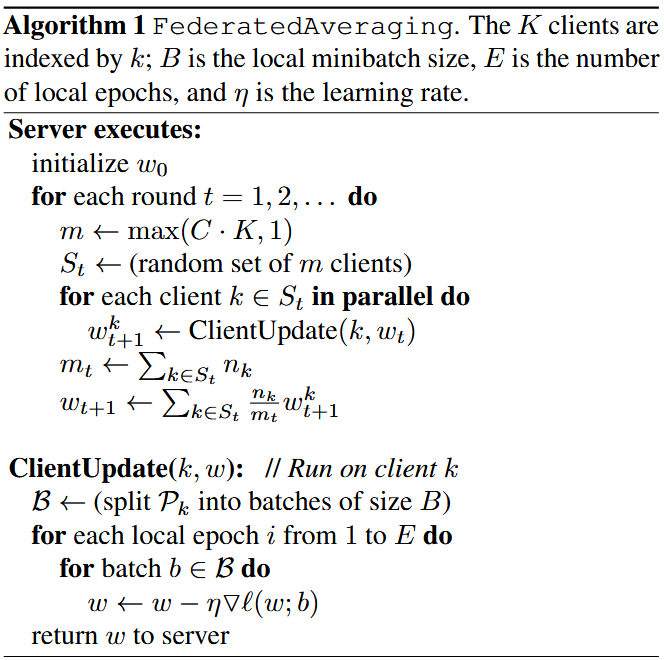
\includegraphics[width=0.40\linewidth]{images/Federated averaging.png}
  \end{center}
\end{frame}

% =======================
\begin{frame}{Problema: média convencional sob ataque bizantino}
  Na agregação por média, um nó bizantino pode enviar um gradiente que:
  \begin{itemize}
    \item tem \textbf{alta magnitude}
    \item aponta na \textbf{direção oposta}
  \end{itemize}

  \vspace{0.6em}
  \begin{center}
    % Ajuste o caminho conforme seu projeto
    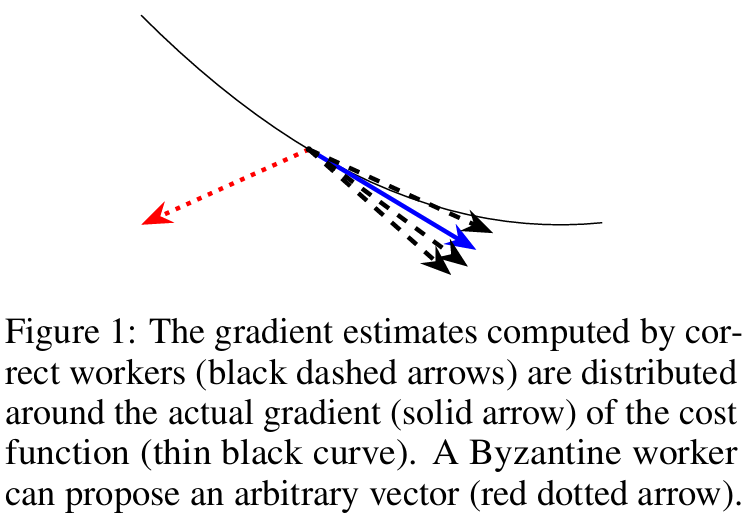
\includegraphics[width=0.40\linewidth]{images2/agregacao_media_erro.png}
  \end{center}
\end{frame}

% =======================
\begin{frame}{Intuição: gradientes honestos vs. maliciosos}
  Gradientes honestos:
  \begin{itemize}
    \item são \textbf{ruidosos} por causa dos mini-batches
    \item tendem a ser \textbf{próximos} entre si 
  \end{itemize}

  \vspace{0.6em}
  Gradientes maliciosos:
  \begin{itemize}
    \item desviam a atualização global para \textbf{não convergir}
    \item exploram a sensibilidade da média a aoutliers
  \end{itemize}
\end{frame}

% =======================
\section{Krum / Multi-Krum}

\begin{frame}{Algoritmo de Krum}
  Krum busca um agregador robusto a nós bizantinos:

  \vspace{0.4em}
  \begin{itemize}
    \item (i) Não ser enganado por outliers
    \item (ii) Não descartar gradientes honestos em excesso
  \end{itemize}

  \vspace{0.8em}
  Objetivo: gerar um gradiente agregado \(g\) que
  \begin{itemize}
    \item aponte para uma direção correta
    \item não exploda em magnitude
  \end{itemize}

  \[
    \langle \mathbb{E}[F], g\rangle \ge (1-\sin\alpha)|g|^2
  \]
\end{frame}

% =======================
\begin{frame}{Krum: ideia central}

    \begin{itemize}
        \item Não combina todos os vetores em um só.
        \item Seleciona um gradiente que pareça certo e com uma boa vizinhança
    \end{itemize}

\end{frame}

% =======================
\begin{frame}{Krum: algoritmo}
  Dados vetores de gradientes \(V_1,\dots,V_n\):

  \vspace{0.3em}
  \begin{enumerate}
    \item Calcule as distâncias para todos os pares:
    \[
      \lVert V_i - V_j \rVert^2 \quad \forall j\neq i
    \]
    \item Para cada \(i\), selecione os \(n-f-2\) vizinhos mais próximos e chame de \(N_i\)
    \item Score:
    \[
      s(i) = \sum_{j\in N_i}\lVert V_i - V_j \rVert^2
    \]
    \item Escolha:
    \[
      \arg\min_i\; s(i)
    \]
  \end{enumerate}

  \vspace{0.4em}
  Custo: \(O(n^2\cdot d)\) (nós \(\times\) dimensão do gradiente).
\end{frame}

% =======================
\begin{frame}{Multi-Krum}
  Escolher um único gradiente pode desacelerar o treino.

  \vspace{0.6em}
  \textbf{Multi-Krum}:
  \begin{itemize}
    \item Seleciona até \(m\) vetores com menores scores
    \item Faz a média desses \(m\) vetores
  \end{itemize}

  \vspace{0.4em}
  Casos extremos:
  \begin{itemize}
    \item \(m=1\) \(\Rightarrow\) Krum
    \item \(m=n\) \(\Rightarrow\) média convencional
  \end{itemize}
\end{frame}

% =======================
\begin{frame}{O que o Krum resolve (e o que não resolve)}
  \textbf{Resolve bem:}
  \begin{itemize}
    \item outliers aleatórios
    \item ataques de grande magnitude que puxam a média
  \end{itemize}

  \vspace{0.6em}
  \textbf{Não verifica:}
  \begin{itemize}
    \item se o gradiente é bom para o treinamento
    \item apenas \textbf{consistência geométrica} (proximidade/distâncias)
  \end{itemize}
\end{frame}

% =======================
\section{Ataque ao Krum}

\begin{frame}{Ataque ao Krum: intuição}
  Objetivo do atacante: Modificar a direção do gradiente sem parecer um outlier.

  \vspace{0.6em}
  Estratégia:
  \begin{itemize}
    \item criar um \textbf{cluster malicioso compacto} (gradientes maliciosos próximos entre si)
    \item ficar \textbf{próximo de alguns gradientes honestos} (explorando o ruído do SGD)
    \item apontar para uma direção \textbf{ruim} mas \textbf{plausível}
  \end{itemize}
\end{frame}

% =======================
\begin{frame}{Por que funciona}
  O Krum procura o vetor com melhor vizinhança.
  Se o atacante garante uma boa vizinhança, então:

  \vspace{0.5em}
  \begin{itemize}
    \item o vetor malicioso \textbf{não é extremo}
    \item fica \textbf{dentro da nuvem} de gradientes
    \item o cluster malicioso é \textbf{muito consistente} \(\Rightarrow\) score pequeno
    \item o Krum pode selecionar o vetor malicioso como “mais confiável”
  \end{itemize}
\end{frame}

% =======================
\section{Peer-to-Peer e SPDL}

\begin{frame}{Peer-to-Peer (P2P): visão geral}
  A comunicação é definida por um \textbf{grafo direcionado}.
  Cada nó mantém e atualiza um modelo local interagindo com seus vizinhos.

  \vspace{0.5em}
  Problemas principais:
  \begin{itemize}
    \item falta de confiança
    \item nós bizantinos
    \item privacidade (gradientes podem vazar informação)
  \end{itemize}
\end{frame}

% =======================
\begin{frame}{SPDL: o que promete}
  SPDL busca combinar:
  \begin{itemize}
    \item \textbf{descentralização} 
    \item \textbf{privacidade} 
    \item \textbf{tolerância a bizantinos} 
    \item \textbf{auditabilidade} (blockchain)
  \end{itemize}
\end{frame}

% =======================
\begin{frame}{SPDL: inicialização}
  \begin{itemize}
    \item Cada nó gera chaves \(PK\) (pública) e \(SK\) (privada) e um id de 256 bits
    \item Cria um bloco gênesis (nó inicial da blockchain)
    \item O nó só participa se tiver registro (pk, id, IP, etc.)
  \end{itemize}

  \vspace{0.4em}
  \textbf{Parâmetros globais (ex.):}
  \begin{itemize}
    \item reputação inicial (popularidade) igual para todos
    \item learning rate, número de rodadas \(T\)
    \item variância do ruído gaussiano
  \end{itemize}
\end{frame}

% =======================
\begin{frame}{SPDL: decisão do líder}

  \begin{figure}
      \centering
      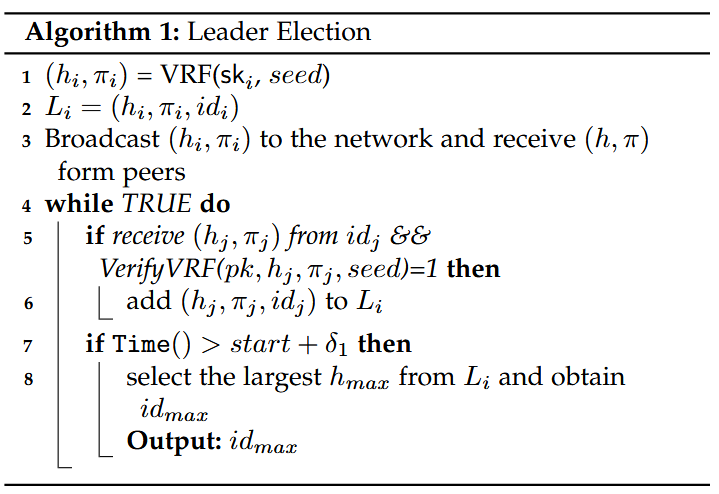
\includegraphics[width=0.5\linewidth]{images2/selecao de lider.png}
  \end{figure}

  \vspace{0.5em}
  Intuição de segurança: não é possível forjar \(h\) e \(\pi\) para outros nós.
\end{frame}

% =======================
\begin{frame}{SPDL: cálculo do gradiente com privacidade}
  Cada nó:
  \begin{itemize}
    \item calcula SGD localmente
    \item adiciona \textbf{ruído gaussiano} ao gradiente
    \item transmite o gradiente ruidoso e recebe o dos outros
  \end{itemize}
\end{frame}

% =======================
\section{Consenso em blockchain (BFT)}

\begin{frame}{SPDL: consenso BFT em quatro fases}
  Em vez de Proof-of-Work / Proof-of-Stake, SPDL usa um consenso \textbf{BFT}.

  \vspace{0.6em}
  Fases:
  \begin{enumerate}
    \item \textbf{PRE-PREPARE}
    \item \textbf{PREPARE}
    \item \textbf{COMMIT}
    \item \textbf{DECIDE}
  \end{enumerate}
\end{frame}

\begin{frame}{PRE-PREPARE}
    \begin{figure}
        \centering
        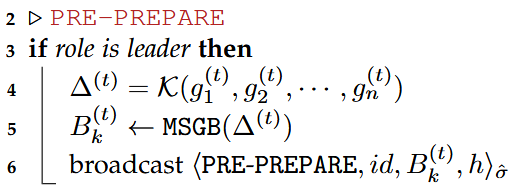
\includegraphics[width=0.75\linewidth]{images2/pre-prepare.png}
    \end{figure}
\end{frame}

\begin{frame}{PREPARE}
    \begin{figure}
        \centering
        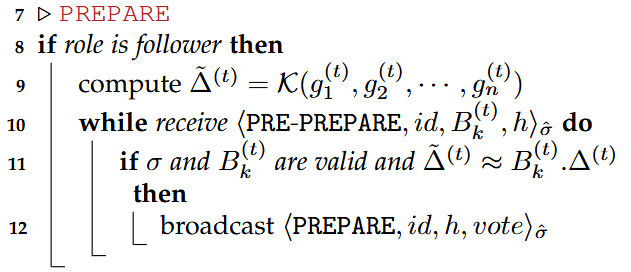
\includegraphics[width=0.75\linewidth]{images2/prepare.png}
    \end{figure}
\end{frame}

\begin{frame}{COMMIT}
    \begin{figure}
        \centering
        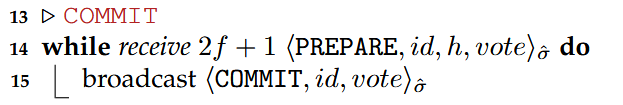
\includegraphics[width=0.75\linewidth]{images2/commit.png}
    \end{figure}
\end{frame}

\begin{frame}{DECIDE}
    \begin{figure}
        \centering
        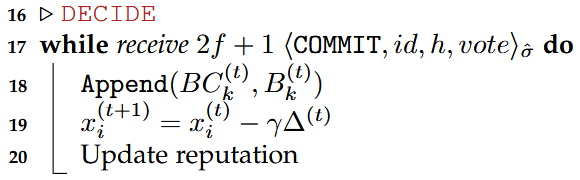
\includegraphics[width=0.75\linewidth]{images2/decide.png}
    \end{figure}
\end{frame}

% =======================
\begin{frame}{Por que blockchain ajuda}
  \textbf{Vantagens:}
  \begin{itemize}
    \item só entra no histórico o que recebeu \textbf{quórum} e foi verificado
    \item histórico imutável
    \item permite \textbf{auditar} e \textbf{punir} nós suspeitos (reduzindo reputação)
  \end{itemize}

  \vspace{0.6em}
  \textbf{Efeito do papel de líder:}
  \begin{itemize}
    \item menos dependência dos outros para avançar
    \item menor risco de ficar para trás
    \item maior controle do ritmo de treino
  \end{itemize}
\end{frame}

\begin{frame}{Referências}
    \begin{itemize}
        \item Byzantine Machine Learning: A Primer - Guerraoui et al., 2024
        \item Machine Learning with Adversaries: Byzantine Tolerant Gradient Descent - Blanchard et al., 2017
        \item Local Model Poisoning Attacks to Byzantine-Robust Federated Learning - Fang et al., 2020
        \item SPDL: Blockchain-secured and Privacy-preserving Decentralized Learning - Xu et al., 2022
    \end{itemize}
\end{frame}

% =======================
\begin{frame}
  \centering
  \Huge Obrigado
\end{frame}

\end{document}
